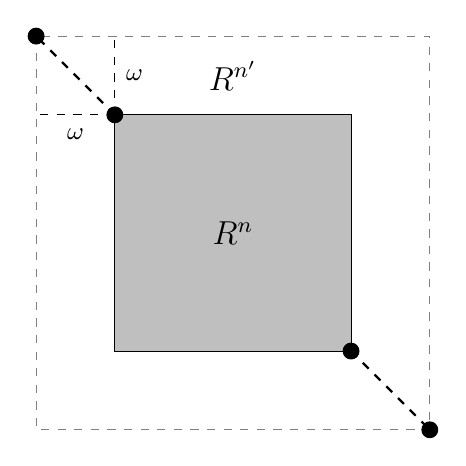
\begin{tikzpicture}[scale=.5]

%set up some coordinates 
%-----------------------
\coordinate (C1) at (0,10); % Outer top left
\coordinate (C2) at (10,0); % Outer bottom right
\coordinate (C3) at (2,8); % Inner top left
\coordinate (C4) at (8,2); % Inner bottom right

%draw figure contents
%--------------------

\draw [fill=lightgray] (C3) rectangle (C4); % Inner rectangle
\draw[dashed, color=gray] (C1) rectangle (C2); % Outer rectangle

\draw [fill] (C1) circle [radius=0.2]; % Outer top left
\draw [fill] (C2) circle [radius=0.2]; % Outer bottom right
\draw [fill] (C3) circle [radius=0.2]; % Inner top left
\draw [fill] (C4) circle [radius=0.2]; % Inner bottom right

\draw[thick,dashed] (C3) -- (C1); % Inner top left to outer top left
\draw[thick,dashed] (C4) -- (C2); % Inner bottom right to outer bottom right

\draw[dashed] (C3) -- (0,8);
\draw[dashed] (C3) -- (2,10);

\draw (5,5) node {\large $R^n$};
\draw (5,9) node {\large $R^{n'}$};

\draw (1,7.5) node {\small $\omega$}; % x1-w
\draw (2.5,9) node {\small $\omega$}; % y1-w

\end{tikzpicture}